\documentclass[paper=a4,fontsize=11pt]{scrartcl} % KOMA-article class




%\usepackage[1-5]{pagesel}
\usepackage[ngerman]{babel}
%for german quotations
\let\oldquote'
\newif\ifquoteopen
\catcode`\'=\active
\makeatletter
\DeclareRobustCommand*{'}{%
   \@ifnextchar'{%
     \ifquoteopen
       \global\quoteopenfalse\grqq\expandafter\@gobble
     \else
       \global\quoteopentrue\glqq\expandafter\@gobble
     \fi
   }{\oldquote}%
}
\makeatother

\usepackage[utf8]{inputenc}
\usepackage[protrusion=true,expansion=true]{microtype}
\usepackage{amsmath,amsfonts,amsthm}     % Math packages
\usepackage{graphicx}                    % Enable pdflatex
\usepackage[svgnames]{xcolor}            % Colors by their 'svgnames'
\usepackage{geometry}
	%\textheight=700px                    % Saving trees ;-)
%\usepackage{url}
\usepackage[colorlinks=true,
linkcolor=blue,
urlcolor=blue]{hyperref}
\usepackage{float}
\usepackage{etaremune}
\usepackage{wrapfig}
\usepackage{bibentry}
\nobibliography*
\usepackage{natbib}
%\bibliographystyle{unsrtnat}
\usepackage{attachfile}
%\usepackage{biblatex}
\usepackage[babel, german=quotes]{csquotes}
\frenchspacing              % Better looking spacings after periods
%%\pagestyle{empty}           % No pagenumbers/headers/footers

%\addtolength{\voffset}{-40pt}
%\addtolength{\textheight}{20pt}

\setlength\topmargin{0pt}
\addtolength\topmargin{-\headheight}
\addtolength\topmargin{-\headsep}
\setlength\oddsidemargin{0pt}
\setlength\textwidth{\paperwidth}
\addtolength\textwidth{-2in}
\setlength\textheight{\paperheight}
%\addtolength\textheight{-3in}
\addtolength\textheight{-2in}
\usepackage{layout}

%%% Custom sectioning}{sectsty package)
%%% ------------------------------------------------------------
\usepackage{sectsty}

\sectionfont{%			            % Change font of \section command
	\usefont{OT1}{phv}{b}{n}%		% bch-b-n: CharterBT-Bold font
	\sectionrule{0pt}{0pt}{-5pt}{3pt}}

%%% Macros
%%% ------------------------------------------------------------
\newlength{\spacebox}
\settowidth{\spacebox}{8888888888}			% Box to align text
\newcommand{\sepspace}{\vspace*{1em}}		% Vertical space macro

\newcommand{\MyName}[1]{ % Name
		\huge \usefont{OT1}{phv}{b}{n} \hfill #1
		\par \normalsize \normalfont}
		
\newcommand{\MySlogan}[1]{ % Slogan}{optional)
		\large \usefont{OT1}{phv}{m}{n}\hfill \textit{#1}
		\par \normalsize \normalfont}

\newcommand{\NewPart}[2]{\section*{\uppercase{#1} #2}}

\newcommand{\PersonalEntry}[2]{
		\noindent\hangindent=2em\hangafter=0 % Indentation
		\parbox{\spacebox}{        % Box to align text
		\textit{#1}}		       % Entry name}{birth, address, etc.)
		\hspace{1.5em} #2 \par}    % Entry value

\newcommand{\SkillsEntry}[2]{      % Same as \PersonalEntry
		\noindent\hangindent=2em\hangafter=0 % Indentation
		\parbox{\spacebox}{        % Box to align text
		\textit{#1}}			   % Entry name}{birth, address, etc.)
		\hspace{1.5em} #2 \par}    % Entry value	
		
\newcommand{\EducationEntry}[4]{
		\noindent \textbf{#1} \hfill      % Study
		\colorbox{White}{%
			\parbox{6em}{%
			\hfill\color{Black}#2}} \par  % Duration
		\noindent {#3} \par        % School
		\noindent\hangindent=2em\hangafter=0  #4 % Description
		\normalsize \par}

\newcommand{\WorkEntry}[4]{				  % Same as \EducationEntry
		\noindent \textbf{#1} \hfill      % Jobname
		\colorbox{White}{\color{White}#2} \par  % Duration
		\noindent \textit{#3} \par              % Company
		\noindent\hangindent=2em\hangafter=0 \small #4 % Description
		\normalsize \par}


        
\newcommand{\FundingEntry}[4]{
        \noindent #1: \textit{#2} (#3, #4).}

\newcommand{\TalkEntry}[4]{
		\noindent #1, #2, #3 #4}

\newcommand{\ThesisEntry}[5]{
		\noindent #1 -- #2 #3 \textit{#4} #5}

\newcommand{\CourseEntry}[3]{
		\noindent \item{#1: \textit{#2} #3}}

%%% Begin Document
%%% ------------------------------------------------------------
\begin{document}

\bibliographystyle{unsrtnat}
\nobibliography{publ}

%\layout

% you can upload a photo and include it here...
% \begin{wrapfigure}{l}{0.5\textwidth}
% 	\vspace*{-2em}
% 		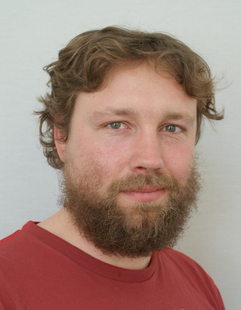
\includegraphics[width=0.2\textwidth]{julian.png}
% \end{wrapfigure}

\MyName{Julian Sagebiel}
\MySlogan{\vspace{-0.2in}\begin{flushright}Department of Economics\\Swedish University of Agricultural Sciences, Uppsala \\
\href{mailto:julian.sagebiel@slu.se}{julian.sagebiel@slu.se}\\
\href{https://www.slu.se/en/ew-cv/julian-sagebiel/}{slu.se}
\end{flushright}}

\sepspace
 \NewPart{Überblick}{}
 Ich bin Researcher am Department of Economics der Swedish University of Agricultural Sciences und befasse mich insbesondere mit Konsumentenverhalten und der Bewertung nicht-gehandelter Güter im Umwelt- und Agrarsektor. 
%%% Personal details
%%% ------------------------------------------------------------
% \NewPart{Personal Details}{}

% \PersonalEntry{Postal Address}{ Technische Universität Berlin EB 4-2, Straße des 17. Juni 145, D-10623 Berlin, EB 4-2 }
% \PersonalEntry{Marital Status}{not married, 1 daughter, 2 sons}
% \PersonalEntry{Date of Birth}{August, 12, 1983}
% \PersonalEntry{Place of Birth}{Berlin}


%%% Work experience
%%% ------------------------------------------------------------
\NewPart{Akademische Laufbahn}{}

% \noindent \textbf{Professor of Physics} \hfill      % Study
% 		\colorbox{White}{%
% 			\parbox{6em}{%
% 			\hfill\color{Black}2016-$\qquad$}} \par
\EducationEntry{Researcher}{Seit 2020}{Swedish University of Agricultural Sciences}
{\begin{itemize}
\item{Entscheidungsverhalten von Landwirten und Konsumenten}
\item{Ökonomische Experimente (z.B. Öffentliche-Gut Spiele) und Discrete Choice Experimente}
\item{Mitarbeit in verschiedenen trans- und interdisziplinären Forschungsprojekten auf nationaler und EU Ebene} 
\end{itemize}}
\sepspace

\EducationEntry{Wissenschaftlicher Mitarbeiter}{2017-2020}{Technische Universität Berlin}
{\begin{itemize}
\item{Umweltökonomik und Verbraucherverhalten}
\item{Mikroökonometrie und  diskrete Entscheidungsmodelle}
\item{Lehraufgaben: Studienprojekte für Master- und Bachlorstudierende in Umweltökonomik und Statstik}
\end{itemize}}
\sepspace

\EducationEntry{Wissenschaftler Mitarbeiter}{2013-2017}{Institut für ökologische Wirtschaftsforschung Berlin}{\begin{itemize}\item{Transdisziplinäre Forschung in Land- und Wassermanagement} \item{Empirische Forschung zur ökonomischen Bewertung nicht-gehandelter Güter} \item{Design und Auswertung von Umfragen}\end{itemize}}
\sepspace
\EducationEntry{Wissenschaftlicher Mitarbeiter}{2009-2013}{Humboldt-Universität zu Berlin}
{\begin{itemize}\item{Forschung zu nachhaltigen Megastädten} \item {Ökonomische Bewertung nicht-gehandelter Güter des Energiesektors in Ländern des Globalen Südens} 
\item{Leitung eines Projekts zur Steigerung der Energieeffizienz in der indischen Landwirtschaft}\end{itemize}}


\sepspace
%%% Education
%%% ------------------------------------------------------------
\NewPart{Ausbildung}{}

\EducationEntry{Promotion Agrarökonomik}{2011-2017}{Humboldt-Universität zu Berlin}{Titel der Doktorarbeit: \href{https://edoc.hu-berlin.de/handle/18452/18406?locale-attribute=en}{\textit{Valuing improvements in electricity supply using   discrete \newline choice experiments}}\\
Magna Cum Laude. Doktorvater: Prof. Dr. Markus Hanisch}
\sepspace

\EducationEntry{Diplom-Volkswirt}{2003-2008}{Otto-von-Guericke-Universtität Magdeburg}{Titel der Diplomarbeit:  \textit{Motivstruktur des Altruismus unter Effizienzbedingung} \\Note: 1,8 (gut). Betreuer der Diplomarbeit: Prof. Dr. Joachim Weimann}



%\newpage


\NewPart{Forschungsprojekte}{}

\begin{etaremune}

\item\FundingEntry {Europäische Union Horizon 2020}{\href{}{AgriFoodBoost: Boosting Excellence in Experimental Research for Agri-Food Economics and Management}}{Wissenschaftlicher Mitarbeiter}{2020-2023}

\item\FundingEntry {Swedish research council for sustainable development (FORMAS)}{\href{https://www.slu.se/en/departments/soil-environment/research/agricultural-water-management-/extreme-weather-and-resilience-in-swedish-agriculture/}{Extreme weather: Risks and solutions to increase the resilience of the Swedish agricultural production}}{Wissenschaftlicher Mitarbeiter}{2020-2022}

\item\FundingEntry {Europäische Union Horizon 2020}{\href{www.project-contracts20.eu}{Contracts2.0: Co-design of novel contract models for innovative agri-environmental-climate measures and for
valorisation of environmental public goods within the value chain}}{Wissenschaftlicher Mitarbeiter}{2019-2023}


\item\FundingEntry {Bundesministerium für Bildung und Forschung}{\href{https://www.ioew.de/projekt/pado_prozesse_und_auswirkungen_von_duenendurchbruechen_an_der_deutschen_ostseekueste/}{PADO – Prozesse und Auswirkungen von Dünendurchbrüchen an der deutschen Ostseeküste}}{Wissenschaftlicher Mitarbeiter}{2016-2018}

\item\FundingEntry {Bundesministerium für Bildung und Forschung}{\href{https://www.ioew.de/projekt/stadtgruen_wertschaetzen/}{Stadtgrün – Bewertung, Management und Kommunikation als Schlüssel für eine klimaresiliente und naturnahe Grünflächen- entwicklung}}{Wissenschaftlicher Mitarbeiter}{2016-2018}


\item\FundingEntry {Bundesministerium für Bildung und Forschung}{\href{https://www.ioew.de/projekt/innovative_systemloesungen_fuer_ein_transdisziplinaeres_und_regionales_oekologisches_hochwasserrisikoman/}{In\_StröHmunG – Innovative Systemlösungen für ein transdisziplinäres und regionales ökologisches Hochwasserrisikomanagement und naturnahe Gewässerentwicklung}}{Wissenschaftlicher Mitarbeiter}{2015-2018}

\item\FundingEntry {Bundesministerium für Bildung und Forschung}{\href{https://secos.deutsche-kuestenforschung.de/}{SECOS – Die Leistung der Sedimente in deutschen Küstenmeeren}}{Wissenschaftlicher Mitarbeiter}{2013-2016}

\item\FundingEntry {Bundesministerium für Bildung und Forschung}{\href{https://www.cc-landstrad.de/}{CC-LandStraD – Strategien für eine nachhaltige Landnutzung im Zeichen des Klimawandels für Deutschland}}{Wissenschaftlicher Mitarbeiter}{2013-2016}

\item\FundingEntry {Bundesministerium für Bildung und Forschung}{\href{http://www.klimzug-radost.de/en/info}{RA:dOst – Regionale Anpassungsstrategien für die deutsche Ostseeküste}}{Wissenschaftlicher Mitarbeiter}{2013-2014}


\item\FundingEntry {DZ BANK-Stiftung}{\href{https://www.agrar.hu-berlin.de/de/institut/departments/daoe/koopwiss/forschung/energeno}{ENERGENO – Ist genossenschaftlicher Strom mehr wert? Zur Zahlungsbereitschaft für genossenschaftlichen Strom}}{Wissenschaftlicher Mitarbeiter}{2012-2015}

\item\FundingEntry {Europäische Kommission}{\href{https://ec.europa.eu/agriculture/external-studies/support-farmers-coop_en}{Support for Farmers’ Cooperatives}}{Berater}{2011-2012}

\item\FundingEntry {Bundesministerium für Bildung und Forschung}{\href{https://www.iaaw.hu-berlin.de/de/hip/institutes/resecon}{Sustainable Hyderabad - Climate and Energy in a Complex Transition Process towards Sustainability in Hyderabad - Mitigation and Adaptation Strategies by Changing Institutions, Governance Structures, Lifestyles and Consumption Patterns}}{Wissenschaftlicher Mitarbeiter}{2009-2013}

\end{etaremune}




% \NewPart{Seminars and Colloquia}{}
% \begin{etaremune}
% \item\TalkEntry{Assistant Secretary of Defense for Research \& Engineering}{Basic Research Forum}{4/21/16}{}

% \item\TalkEntry{Rensselaer Polytechnic Institute}{Physics colloquium}{9/24/03}{}
% \end{etaremune}


\NewPart{Lehre}{}

\begin{etaremune}
\item[]
\vspace{-24pt}

\CourseEntry{Oktober 2021}{Hands-on workshop on statistical tools in social and economic sciences applied to agriculture, food and the environment}{University of Zagreb}

\CourseEntry{Wintersemester 2020 and 2021}{Vorlesung: Experimental methods for economics and business studies}{Swedish University of Agricultural Sciences, Uppsala}

\CourseEntry{2017 to 2020}{Verschiedene Einzelvorlesungen in den Lehrveranstaltungen Landschaftsökonomie I und II}{Technische Universität Berlin}

\CourseEntry{Wintersemester 2019/20 und Sommersemester 2020}{Studienprojekt: Experimente als Entscheidungsgrundlage landschaftsplanerischer Prozesse}{Technische Universität Berlin}

\CourseEntry{Summer Term 2019}{Studienprojekt: Ökosystemleistungen in Auen}{Technische Universität Berlin}

\CourseEntry{Wintersemester 2018/19}{Studienprojekt: Rethinking Urban Space: The Demand for Green Infrastructure}{Technische Universität Berlin}

\CourseEntry{Oktober 2018}{Autumn School: Infrastructure Research and Policy Training (InfraTrain) -- Methodical Track Discrete Choice Experiments}{ Deutsches Insititut für Wirtschaftsforschung (DIW), Berlin}

\CourseEntry{Sommersemester 2018}{Studienprojekt: Angewandte statistische Methoden für die Landschaftsplanung}{Technische Universität Berlin}

\CourseEntry{Wintersemester 2017/18}{Studienprojekt: The Recreational Value of Urban Green}{Technische Universität Berlin}

\CourseEntry{September 2017}{Summer School: Using Discrete Choice Experiments for the Economic Valuation of Ecosystem Services in Rural Landscapes}{Leibniz-Zentrum für Agrarlandschaftsforschung (ZALF)}

\CourseEntry{März 2017}{Workshop: Methods for Cooperative Sciences -- Methodical Track Discrete Choice Experiments}{Humboldt-Universität zu Berlin}


\CourseEntry{Sommersemester 2015}{Seminar: Ökonomische Bewertung von Umwelt- und Energiegütern -- Umfragebasierte Methoden und Theorie}{Humboldt-Universität zu Berlin}

\CourseEntry{Februar 2015}{Promotionsseminar: Quantitative Methoden}{International School of Management, Dortmund}

\CourseEntry{Januar 2014}{Seminar: Discrete Choice Experiments -- Theory and Application}{International School of Management, Dortmund}
\end{etaremune}

\NewPart{Betreute Bachelor- und Masterarbeiten}{}
\begin{etaremune}

\item \ThesisEntry{Marc Ringborg}{2021}{Bachelorarbeit}{Status quo effects of information treatments in discrete choice experiments}{Swedish University of Agricultural Sciences}

\item \ThesisEntry{Giovanni Slinn}{2021}{Masterarbeit}{A discrete choice experiment on consumer preferences for tofu characteristics in Germany, Italy, and Sweden}{Swedish University of Agricultural Sciences}

\item \ThesisEntry{Erik Furth}{2021}{Masterarbeit}{Floodplain management through economic valuation: Using farmers' preferences to improve pollution-reduction schemes in Germany}{Technische Universität Berlin}

\item \ThesisEntry{Polina Korneeva}{2021}{Masterarbeit}{Valuation of carbon sequestration and storage under different land-use management scenarios: A case study in the regiopolis region of Rostock}{Technische Universität Berlin}

\item \ThesisEntry{Ronja Schönau}{2021}{Masterarbeit}{Assessing preferences for bicycle infrastructure –
A discrete choice experiment in Seoul, South Korea}{Technische Universität Berlin}

\item \ThesisEntry{Dan Xing}{2020}{Masterarbeit}{Discrete choice experiments to measure the economic value of urban green }{Technische Universität Berlin}

\item \ThesisEntry{Ameneh Larijani}{2020}{Masterarbeit}{More than a cycle track? New bicycle facility as a measure to improve living quality in Berlin}{Technische Universität Berlin}

\item \ThesisEntry{Luisa Rau}{2020}{Masterarbeit}{Is money enough to increase social acceptance of hydropower projects in Southern Chile?}{Technische Universität Berlin}

\item \ThesisEntry{Marisa Ramos Rocha}{2020}{Masterarbeit}{Understanding the use of knowledge in decision-making processes to implement nature-based solutions}{Technische Universität Berlin}

\item \ThesisEntry{Jessica Weir and Daniel Soto}{2020}{Masterarbeit}{Willingness to pay for sustainable tourism}{Technische Universität Berlin}

\item \ThesisEntry{Bradyn Winiarski}{2020}{Masterarbeit}{How Valid is Valid Enough? A Review on Validity of Contingent Valuation for Damage Assessments}{Technische Universität Berlin}

\item \ThesisEntry{Yuhan Miao}{2019}{Masterarbeit}{Stated Preferences on the Value of Urban Green Spaces in Germany: How Does the Survey's Consequentiality Influence the Willingness-To-Pay?}{Technische Universität Berlin}

\item \ThesisEntry{Luisa Rau}{2018}{Bachelorarbeit}{Urbane Gemeinschaftsgärten als Grundlage politisch-planerischer Entscheidungen – Eine kontingente Bewertung}{Technische Universität Berlin}

\item \ThesisEntry{Katarzyna Malinowska}{2018}{Masterarbeit}{The Future of Energy Cooperatives in Germany: Exploring strategic alliances with commercial energy companies}{Humboldt-Universität zu Berlin}

\item \ThesisEntry{Sarah Vitone}{2018}{Masterarbeit}{The Value of Urban Gardens}{Technische Universität Berlin}

\item \ThesisEntry{Snigdha Sunil Kunder}{2018}{Masterarbeit}{Assessing the economic value of the conservation of common toads using a willingness to pay survey}{Technische Universität Berlin}

\item \ThesisEntry{Maria Lindow}{2016}{Masterarbeit}{The Role of Cultural Ecosystem Services for the Acceptence of the Local Population with Respect to the Water Framework Directive}{Universität Greifswald}

\item \ThesisEntry{Amely Gundlach}{2016}{Masterarbeit}{Overcoming the Tenant Landlord Dilemma:
An Investigation of the Impact of Cooperative Ownership on the Capitalization of Energy Efficiency}{Humboldt-Universität zu Berlin}


\end{etaremune}

\NewPart{Aktivitäten und Mitgliedschaften}{}
\begin{itemize}





\item  \EducationEntry{\href{https://sites.google.com/view/reecap}{REECAP - A Research Network on Economic Experiments for the Common \newline Agricultural Policy}} {Seit 2016}{Mitglied im akademischen Beirat}


\item \EducationEntry{\href{https://www.agrar.hu-berlin.de/de/institut/departments/daoe/koopwiss/ifg}{Institut für Genossenschaftswesen an der Humboldt-Universtität \newline zu Berlin }}{Seit 2018}{Mitglied im akademischen Beirat}


\item \EducationEntry{\href{https://www.eaere.org/}{European Association of Environmental and Resource \newline Economists }}{Seit 2016}{Mitglied}

\item \EducationEntry{\href{http://www.envecho.com/index.html}{ENVECHO - A scientific network of researchers using \newline Discrete Choice Modelling in the field of environmental valuation}}{Seit 2016}{Mitglied}

\item \EducationEntry{\href{http://www.eaae.org/}{European Association of Agricultural Economists}}{Seit 2016}{Mitglied}

\item \EducationEntry{\href{http://forschungsnetzwerk-energiegenossenschaften.de}{Forschungsnetzwerk Energiegenossenschaften}}{2014-2016}{Gründungsmitglied und Sprecher}{mit Sarah Debor und Jakob Müller}




\end{itemize}


\NewPart{Weitere Aktivitäten}{}
\begin{itemize}
\item \EducationEntry{\href{http://www.eaere-conferences.org/index.php?p=60}{EAERE Conference 2017 Workshop \textit{Spatial Dimensions of \newline Stated Preferences}}}{2016-2017}{Organisator}{mit Klaus Glenk, Robert Johnston und Jürgen Meyerhoff}

\item
\EducationEntry{\href{https://link.springer.com/journal/10640/volumes-and-issues/75-2}{Sonderausgabe \textit{Spatial Dimensions of Stated Preferences}}}{ 2018-2020}{Mitherausgeber Environmental and Resource Economics}{mit Klaus Glenk, Robert Johnston und Jürgen Meyerhoff}

\item 
\EducationEntry{\href{http://www.landschaftsoekonomie.tu-berlin.de/menue/berlin_dce_colloquium/}{Berlin Discrete Choice Colloquium}}{Seit 2016}{Gründungsmitglied und Organisator}{mit Jürgen Meyerhoff}


\item \EducationEntry{\href{http://communications.ext.zalf.de/sites/dce/SitePages/DCE\%20Summer\%20School.aspx}{Summer School \textit{Using Discrete Choice Experiments for the \newline Economic Valuation of Ecosystem Services in Rural Landscapes}}}{2016-2017}{Organisator und Dozent}{mit Kati Haefner, Jürgen Meyerhoff und Jens Rommel}

\item \EducationEntry{\href{https://www.ica-berlin2019.hu-berlin.de/de}{ICA-CCR European Research Conference 2019}}{2018-2019}{Mitglied des wissenschaftlichen Komitees}

\item \EducationEntry{Wissenschaftliche Beratung}{Seit 2012}{Survey Engine GmbH ($>100$h), International School of Management gGmbH ($>50$h), Europäische Kommission ($>40$h), Seminar für Ländliche Entwicklung an der Humboldt-Universität zu Berlin ($>30$h)}{}

\end{itemize}



 \NewPart{Preise und Auszeichnungen}{}
 \begin{itemize}
\item 2017 \href{https://www.agrar.hu-berlin.de/de/institut/departments/daoe/koopwiss/ifg/forschung/wissenschaftlicher-nachwuchs/raiffeisen-schulze-delitzsch-foerderpreis}{Raiffeisen - Schulze-Delitzsch-Förderpreis} für die beste Dissertation im Genossenschaftswesen 2016
 \item 2017 Deutscher Akademischer Austauschdienst (DAAD) Reiseförderung für die \textit{Environmental and Resource Economics} Konferenz in Athen, Griechenland
 \item 2016 Deutscher Akademischer Austauschdienst (DAAD) Reiseförderung für die \textit{Environmental and Resource Economics} Konferenz in Zürich, Schweiz
 \item 2007 Deutscher Akademischer Austauschdienst (DAAD) Förderung zum Auslandssemester an der \textit{Macquarie University Sydney}, Australien

\end{itemize}

% \NewPart{Major Departmental Committees Chaired}{}
% \begin{itemize}
% \item Graduate qualifier exam committee, 2016-present (manage authorship of both Classical and Quantum exams each semester)
% \item CME faculty search committee, 2013 (hired V. Manucharyan and J. Williams)
% \item Undergraduate curriculum review committee, 2011 (authored 50+ page report)
% \end{itemize}

%\newpage



\NewPart{Software}{}
Stata (Experte), R (Experte), \LaTeX (Experte),  LIMDEP (fortgeschritten), NGENE (Experte), Latent Gold (Experte), Biogeme (fortgeschritten), Bash (fortgeschritten), Python (Grundkenntnisse), JavaScript (Grundkenntnisse)

\NewPart{Gutachtertätigkeiten für Zeitschriften}{\href{https://publons.com/a/1337890}{[Publons]}}
Ecological Economics (9), Energy Research \& Social Science (5), 
Energy Economics (4), 
Environmental Science and Pollution Research (4),
European Review of Agricultural Economics (3), Journal of Environmental Economics and Management 
(2), 
Energy Policy (1),
 Environmental and Resource Economics (1), Journal of Behavioral and Experimental Economics (1), 
 Journal of Environmental Economics and Policy
(1), Land Use Policy
(1), Scientific Reports
(1), Utilities Policy
(1), Water Resources and Economics (1)

 \NewPart{Referenzen}{}
 \begin{itemize}
 
\item Prof. Jette Bredahl Jacobsen (Professor und stellvertretende Leiterin des Department Food and Resource Economics, University of Copenhagen, Rolighedsvej 23, 1958 Frb. C, \href{mailto:jbj@ifro.ku.dk}{jbj@ifro.ku.dk}, +45 35 33 17 46) 
\item Dr. Klaus Glenk (Gruppenleiter, Sustainable Ecosystems at  Scotland's Rural College, SRUC, West Mains Road, Kings Buildings, Peter Wilson Building, EH9 3JG Edinburgh,  United Kingdom, \href{mailto:klaus.glenk@sruc.ac.uk}{klaus.glenk@sruc.ac.uk})
\item Prof. Mikolaj Czajkowski (Professor und Vizedekan Forschung, Faculty of Economic Sciences, University of Warsaw, Długa 44/50 
00241 Warsaw, Poland, \href{mailto:mc@uw.edu.pl}{mc@uw.edu.pl},
+48 507 056 557)
\end{itemize}

\newpage

%%% Papers
%%% ------------------------------------------------------------

\NewPart{Wissenschaftliche Artikel unter Begutachtung}{}{}



\begin{etaremune}

\item \bibentry{zawojska2021}

\item \bibentry{Welling2021}

\item \bibentry{rogers2021}


\end{etaremune}



\NewPart{Begutachtete Publikationen}{\href{https://scholar.google.de/citations?user=RzdZi_IAAAAJ&hl=de}{[Google Scholar]}}


\begin{etaremune}
\item \bibentry{Giergiczny2021}
\item \bibentry{VILLAMAYORTOMAS2021}
\item \bibentry{rommel2021consumer}
\item \bibentry{sagebiel2020does}
\item \bibentry{sagebiel2020clean}
\item \bibentry{fruth2020discrete}
\item \bibentry{fruth2019economic}
\item \bibentry{villamayor2019bringing}
\item \bibentry{Glenk2019}
\item \bibentry{knoefel2018consumer}
\item \bibentry{gundlach2018investigating}
\item \bibentry{muller2018structural}
\item \bibentry{rayanov2018economic}
\item \bibentry{ghosh2017small}
\item \bibentry{rommel2017preferences}
\item \bibentry{sagebiel_preference_2017}
\item \bibentry{sagebiel_spatially_2017}
\item \bibentry{kimmich_empowering_2016}
\item \bibentry{sagebiel2016economic}
\item \bibentry{rommel_quality_2016}
\item \bibentry{magliocca2015meta}
\item \bibentry{sagebiel_are_2014}
\item \bibentry{sagebiel_preferences_2014}
\item \bibentry{hanisch_coping_2010}



\end{etaremune}



\NewPart{Buchkapitel}{}
\begin{etaremune}
\item \bibentry{Elsasser2021}
\item \bibentry{Yildiz2019}
\item \bibentry{sagebielbuilding2014}
\item \bibentry{kimmich_peri-urban_2013}
\item \bibentry{sagebiel_governance_2013}
\item \bibentry{rommel_nachhaltige_2012}
\end{etaremune}


\NewPart{Bücher}{}
\begin{etaremune}
\item \bibentry{marielenvironmental}
\item \bibentry{sagebiel2017valuing}
\item \bibentry{sagebiel_enhancing_2016}
\item \bibentry{kimmich_methods_2012} 
\end{etaremune}


\newpage
% \bibliographystyle{apalike}
% \bibliography{publ}
\end{document}
